\documentclass{beamer}

\usepackage[brazil]{babel}
\usepackage[utf8]{inputenc}
\usepackage{caption}
\usetheme{Marburg}
\usecolortheme{beaver}
\setbeamertemplate{footline}[frame number]
\setbeamertemplate{caption}[numbered]
\captionsetup{font=scriptsize,labelfont=scriptsize}
\title{Paradigmas de Programação da linguagem LUA}
\subtitle{Projeto Integrador VI - Paradigmas de linguagens de programação}
\author{Mário Sergio e Pedro Martins}
\date{\today}

\begin{document}
\frame{\titlepage}

\section{Introdução}

\begin{frame}[fragile]
\frametitle{Introdução}
\begin{itemize}
\item Este projeto acadêmico se refere ao desenvolvimento de um estudo e pesquisa, relativo aos paradigmas e conceitos da linguagem de programação Lua.
\begin{figure}[!htb]
\centering

\includegraphics[width=0.3\linewidth]{imagens/logo}
\caption{Logo - Lua Org}
\end{figure}
\end{itemize}
\end{frame}

\subsection{Motivações}
\begin{frame}[fragile]
\frametitle{Introdução}
{\bf Motivações}\vspace{0.4cm}
\begin{itemize}
\item[$\Rightarrow$]<1-> Linguagem dinâmica, similar à python, ou seja, de fácil entendimento;
\item[$\Rightarrow$]<2-> Única linguagem criada fora do eixo de países desenvolvidos com relevância internacional;
\item[$\Rightarrow$]<3-> O nicho de aplicação de Lua é muito vasto;
\item[$\Rightarrow$]<4-> Leve, com apenas 20.000 linhas de código C que podem ser construídos em um intérprete executável 182K em um Linux;
\end{itemize}
\end{frame}

\begin{frame}[fragile]
\frametitle{Introdução}
{\bf Motivações}\vspace{0.4cm}
\begin{itemize}
\item[$\Rightarrow$] Portável, é utilizada em qualquer plataforma com um compilador C ANSI. Lua Pode ser usada em:
\pause
\item Microcontroladores;
\item Plataformas móveis;
Consoles de jogos;
\item Navegadores (traduzido para JavaScript);
\item Aplicações de TV digital;
\item Programas de manipulação de imagens.
\end{itemize}
\end{frame}

\begin{frame}[fragile]
\frametitle{Introdução}
{\bf Exemplos de aplicações Lua}\vspace{0.4cm}
\begin{figure}[!htb]
\centering

\includegraphics[width=0.4\linewidth]{imagens/exemplo2}
\caption{teste}
\end{figure}

\begin{figure}[!htb]
\centering
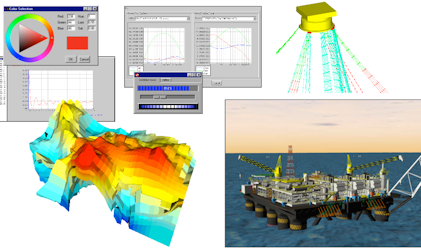
\includegraphics[height=2.5cm]{imagens/exemplo3}
\label{figdroopy}
\quad %espaco separador
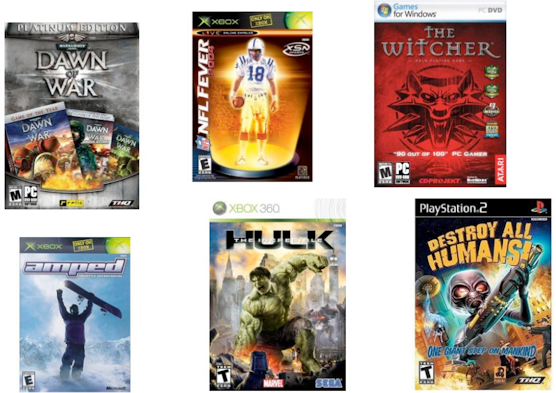
\includegraphics[height=2.5cm]{imagens/exemplo1}
\label{figsnoop}
\caption{Subfiguras}
\label{fig01}
\end{figure}
\end{frame}

\subsection{Objetivos}
\begin{frame}[fragile]
\frametitle{Introdução}
{\bf Objetivos}\vspace{0.4cm}
\begin{itemize}
\item<1-> O objetivo do principal do projeto é aplicar os conhecimentos obtidos na disciplina de paradigmas de linguagem de programação à linguagem LUA.
\begin{itemize}
\item[$\Rightarrow$]<2-> Levantar os paradigmas de programação da linguagem;
\item[$\Rightarrow$]<3-> Analisar Sintaxe e Semântica;
\item[$\Rightarrow$]<4-> Explicar e exemplificar o funcionamento de variáveis. Tipos, sua vinculação, verificação de tipo e escopo;
\item[$\Rightarrow$]<5-> Entender as vantagens, desvantagens e as áreas a qual LUA melhor se aplica;
\item[$\Rightarrow$]<6-> Criação códigos para exemplificar os conceitos apresentados.
\end{itemize}
\end{itemize}
\end{frame}

\section{História}
\begin{frame}[fragile]
\frametitle{História da Linguagem}
{\bf Projeto Inicial}\vspace{0.2cm}
\begin{itemize}
\item[$\Rightarrow$]<1-> A construção da linguagem veio de um projeto entre a PETROBRAS e a PUC-RIO, a fim de produzir um programa de interfaces gráficas para várias aplicações;
\begin{figure}[!htb]
\centering
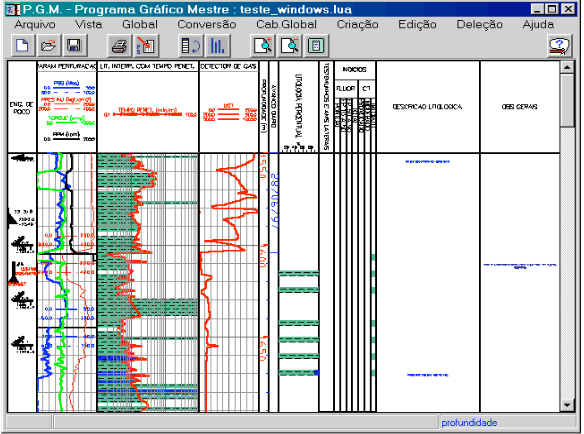
\includegraphics[width=0.3\linewidth]{imagens/imagem1}
\caption{Logo - Lua Org}
\end{figure}
\item[$\Rightarrow$]<2-> Logo surgiu o DEL - Linguagem para Especificação de Diálogos;
\item[$\Rightarrow$]<3-> ‘SOL’ - Simple Object Language, uma linguagem para descrição de objetos,inspirada no bibTex.
\begin{figure}[!htb]
\centering
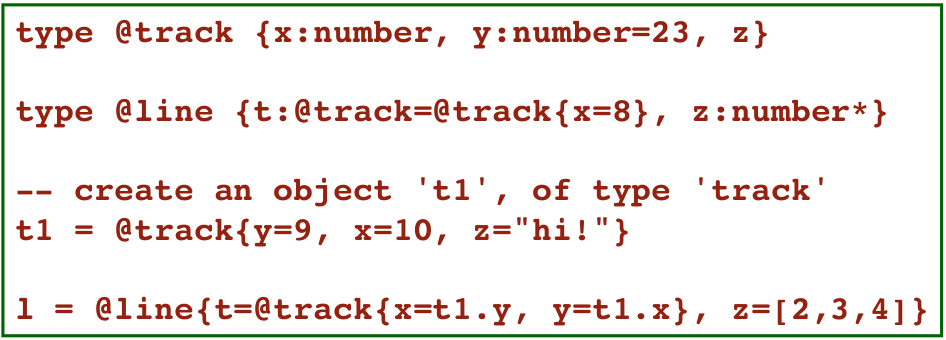
\includegraphics[width=0.3\linewidth]{imagens/imagem2}
\caption{Logo - Lua Org}
\end{figure}
\end{itemize}
\end{frame}

\begin{frame}[fragile]
\frametitle{História da Linguagem}
{\bf Esforço}\vspace{0.2cm}
\begin{itemize}
\item[$\Rightarrow$]<1-> No entanto, DEL e SOL tinha várias limitações como, pouco recurso para construção de diálogos e pouca abstração de dados, se comparadas à linguagens contemporâneas;
\item[$\Rightarrow$]<2-> As propostas de solução era formular uma nova linguagem de configuração genérica com as seguintes características:
\begin{itemize}
\item<3-> Facilmente acoplável;
\item<4-> Portável
\item<5-> Simples e de sintaxe fácil
\end{itemize}
\end{itemize}
\end{frame}

\begin{frame}[fragile]
\frametitle{História da Linguagem}
\begin{itemize}
\item[$\Rightarrow$] O resultado desse projeto foi dado o nome LUA, como um contráste da antiga SOL.
\begin{figure}[!htb]
\centering
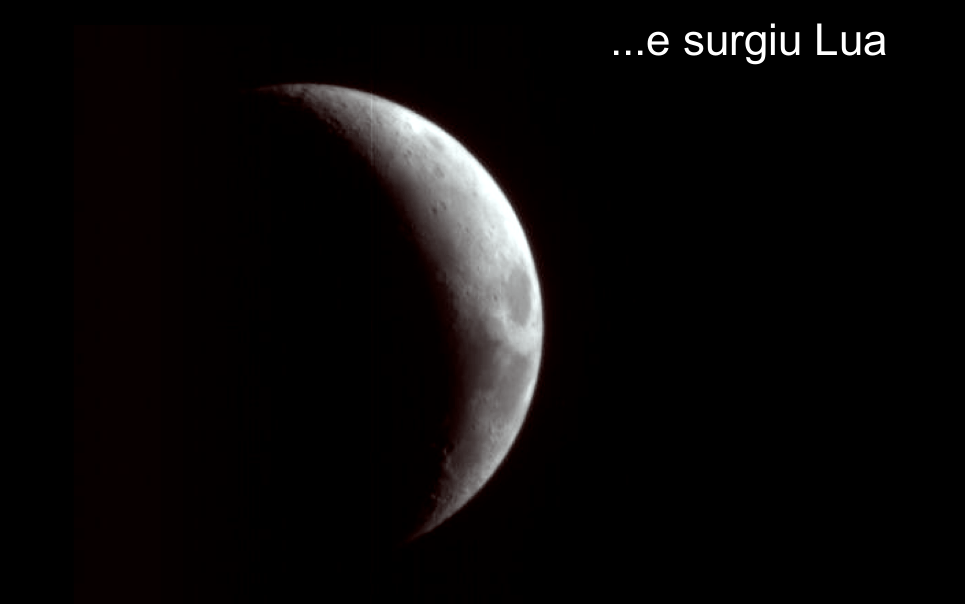
\includegraphics[width=1\linewidth]{imagens/lua}
\caption{Logo - Lua Org}
\end{figure}
\end{itemize}
\end{frame}

\section{Ánálise Léxica e Sintática}
\subsection{Construções léxicas}
\begin{frame}[fragile]
\frametitle{Construções léxicas}
\begin{itemize}
\item Em Lua, os nomes podem ser qualquer cadeia de letras, dígitos, e sublinhados que não começam com um dígito;
\item Os identificadores são usados para nomear variáveis e campos de tabelas;
\item Lua é uma linguagem que diferencia letras minúsculas de maiúsculas;
\item As seguintes cadeias denotam outros itens léxicos: + - * == = <= >= < > = () [] ; : , . .. ...
\item Existem outras construções lexicas, porém estão mais ligadas à convenções da comunidade Lua.
\end{itemize}
\end{frame}

\subsection{Sintaxe}
\begin{frame}[fragile]
\frametitle{Sintaxe}
\begin{itemize}
\item Aqui está a sintaxe completa de Lua na notação BNF estendida. (Ela não descreve as precedências dos operadores).
\begin{figure}[!htb]
\centering
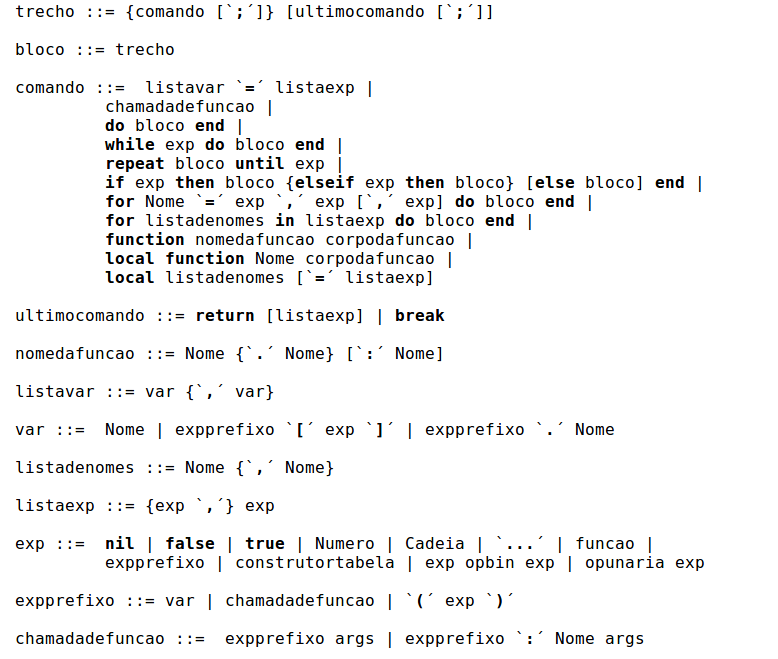
\includegraphics[width=0.9\linewidth]{imagens/sintaxe1}
\end{figure}
\end{itemize}
\end{frame}

\begin{frame}[fragile]
\frametitle{Sintaxe}
\begin{figure}[!htb]
\centering
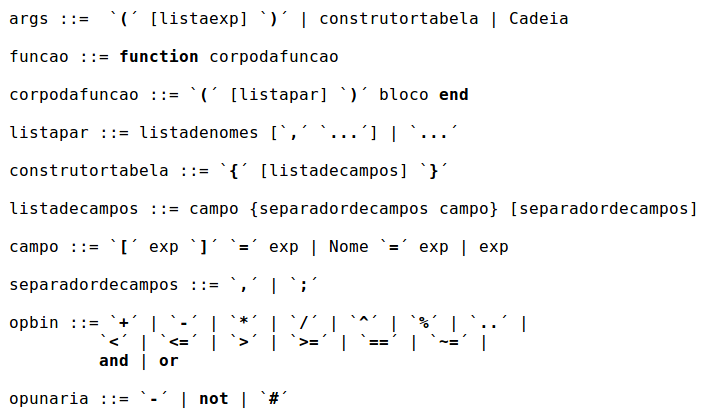
\includegraphics[width=1\linewidth]{imagens/sintaxe2}
\end{figure}
\end{frame}

\section{Semântica das variáveis}
\subsection{Variáveis}
\begin{frame}[fragile]
\frametitle{Variáveis}
\begin{itemize}
\item [$\Rightarrow$]<1-> Em Lua existem três tipos de variáveis, sendo elas as seguites.
\begin{itemize}
\item <2-> Variáveis locais;
\item <3-> Variáveis globais;
\item <4-> Variáveis de tabelas.
\end{itemize}
\item [$\Rightarrow$]<5-> A diferença entre variáveis locais e globais é o uso da palavra reservada ‘local’, antes do nome da variável.
\end{itemize}
\begin{figure}[!htb]
\centering
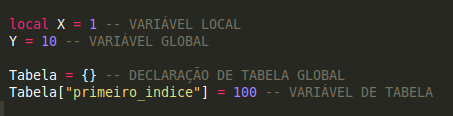
\includegraphics[width=0.7\linewidth]{imagens/variaveis}
\end{figure}
\end{frame}

\subsection{Vinculação}
\begin{frame}[fragile]
\frametitle{Vinculação}
\begin{itemize}
\item<1-> Lua é uma linguagem dinamicamente tipada;
\item<2-> A linguagem trabalha com vinculação dinâmica de tipos;
\item<3-> Existem oito tipos de dados básicos em Lua:
\begin{itemize}
\item<4-> nil - boolean - number - string- thread;
\item<5-> \textbf{function - userdata - table.}
\end{itemize}
\item<6-> O tempo de vida das variáveis é definido pelo fato de ela se global ou local;
\item<7-> Se a variável for local terá o tempo de vida definido pelo tempo de execução do escopo onde se encontra.
\end{itemize}
\end{frame}

\subsection{Verificação de Tipos}
\begin{frame}[fragile]
\frametitle{Verificação de Tipos}
\begin{itemize}
\item A verificação de tipos em Lua é feita em tempo de execução pelo interpretador Lua;
\end{itemize}
\begin{figure}[!htb]
\centering
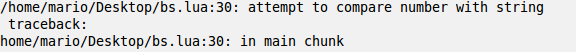
\includegraphics[width=0.3\linewidth]{imagens/verificacao_tipo2}
\caption{Logo - Lua Org}
\end{figure}

\begin{figure}[!htb]
\centering
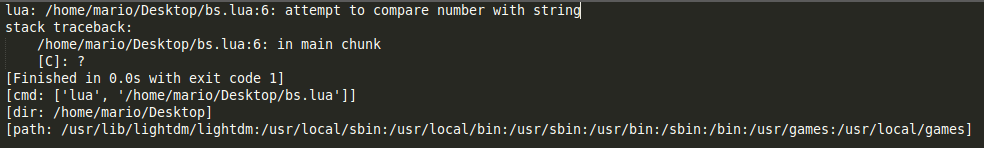
\includegraphics[width=1\linewidth]{imagens/verificacao_tipo}
\caption{Logo - Lua Org}
\end{figure}
\end{frame}

\subsection{Escopo}
\begin{frame}[fragile]
\frametitle{Escopo}
\begin{itemize}
\item<1-> Lua trabalha na modelagem de escopo dinâmico;
\item<2-> Baseia-se na sequência de chamadas de subprogramas;
\item<3-> O escopo pode ser determidado em tempo de execução;
\item<4-> Toda variável é uma variável global a menos que ela seja explicitamente declarada como uma variável local;
\item<5-> Variáveis locais podem ser livremente acessadas por funções definidas dentro do seu escopo ou bloco;
\item<6-> Lua é uma linguagem com escopo léxico.
\end{itemize}
\end{frame}

\end{document}